\documentclass[11pt]{article}
\usepackage[textwidth=18.0cm, textheight=23.0cm, top=2.0cm]{geometry}
\usepackage{pst-all}
\usepackage{amssymb}
\usepackage{tikz}
\usepackage{underscore}\begin{document}
\pagestyle{empty}


ClassName: \underline{\textbf{Class_08.2bp-4}}
\par
BinSize: \underline{\textbf{100 × 100}}
\par
ReduceSize: \underline{\textbf{100 × 100}}
\par
TypeNum: \underline{\textbf{20}}
\par
Num: \underline{\textbf{20}}
\par
OutS: \underline{\textbf{60000}}
\par
InS: \underline{\textbf{41715}}
\par
Rate: \underline{\textbf{0.695}}
\par
UB: \underline{\textbf{6}}
\par
LB0: \underline{\textbf{6}}
\par
LB: \underline{\textbf{6}}
\par
LBWithCut: \underline{\textbf{6}}
\par
NodeCut: \underline{\textbf{0}}
\par
ExtendedNodeCnt: \underline{\textbf{1}}
\par
GenNodeCnt: \underline{\textbf{1}}
\par
PrimalNode: \underline{\textbf{0}}
\par
ColumnCount: \underline{\textbf{6}}
\par
TotalCutCount: \underline{\textbf{0}}
\par
RootCutCount: \underline{\textbf{0}}
\par
LPSolverCnt: \underline{\textbf{1}}
\par
PricingSolverCnt: \underline{\textbf{0}}
\par
BranchAndBoundNum: \underline{\textbf{1}}
\par
isOpt: \underline{\textbf{true}}
\par
TimeOnInitSolution: \underline{\textbf{600.000 s}}
\par
TimeOnPrimal: \underline{\textbf{0.000 s}}
\par
TimeOnPricing: \underline{\textbf{0.000 s}}
\par
TimeOnRmp: \underline{\textbf{0.063 s}}
\par
TotalTime: \underline{\textbf{600.329 s}}
\par
\newpage


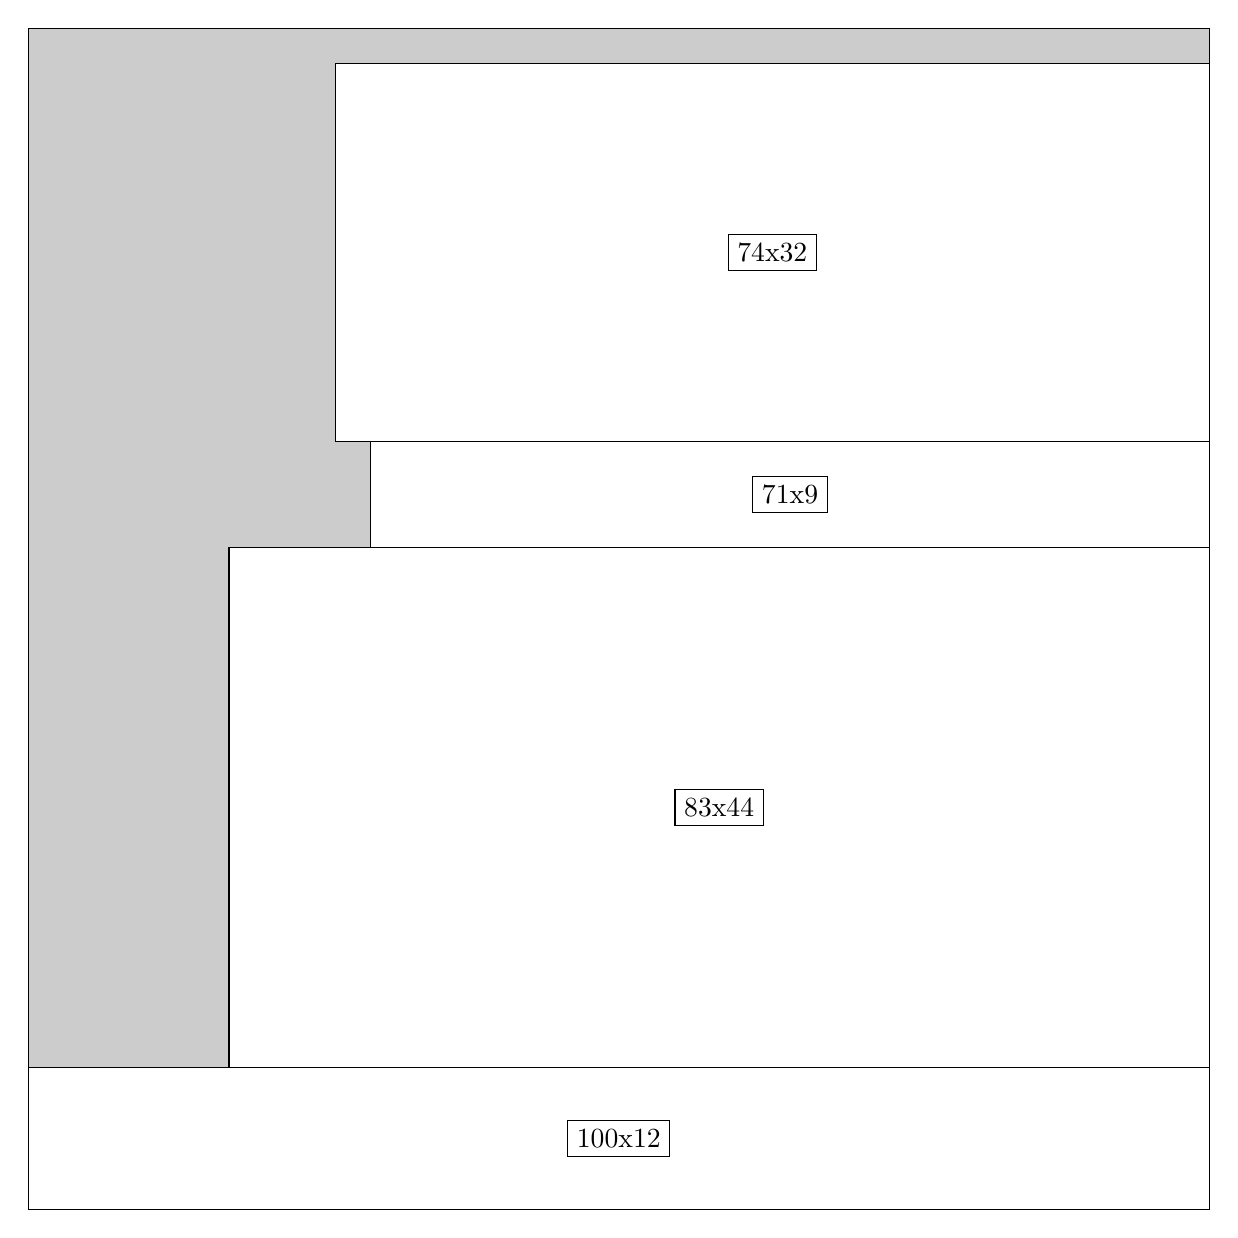
\begin{tikzpicture}[shorten >=1pt,scale=1.0,every node/.style={scale=1.0},->]
\tikzstyle{vertex}=[circle,fill=black!25,minimum size=14pt,inner sep=0pt]
\filldraw[fill=gray!40!white, draw=black] (0,0) rectangle (15.0,15.0);
\foreach \name/\x/\y/\w/\h in {100x12/0.0/0.0/15.0/1.7999999999999998,83x44/2.55/1.7999999999999998/12.45/6.6,71x9/4.35/8.4/10.65/1.3499999999999999,74x32/3.9/9.75/11.1/4.8}
\filldraw[fill=white!40!white, draw=black] (\x,\y) rectangle node[draw] (\name) {\name} ++(\w,\h);
\end{tikzpicture}


w =100 , h =12 , x =0 , y =0 , v =1200
\par
w =83 , h =44 , x =17 , y =12 , v =3652
\par
w =71 , h =9 , x =29 , y =56 , v =639
\par
w =74 , h =32 , x =26 , y =65 , v =2368
\par
\newpage


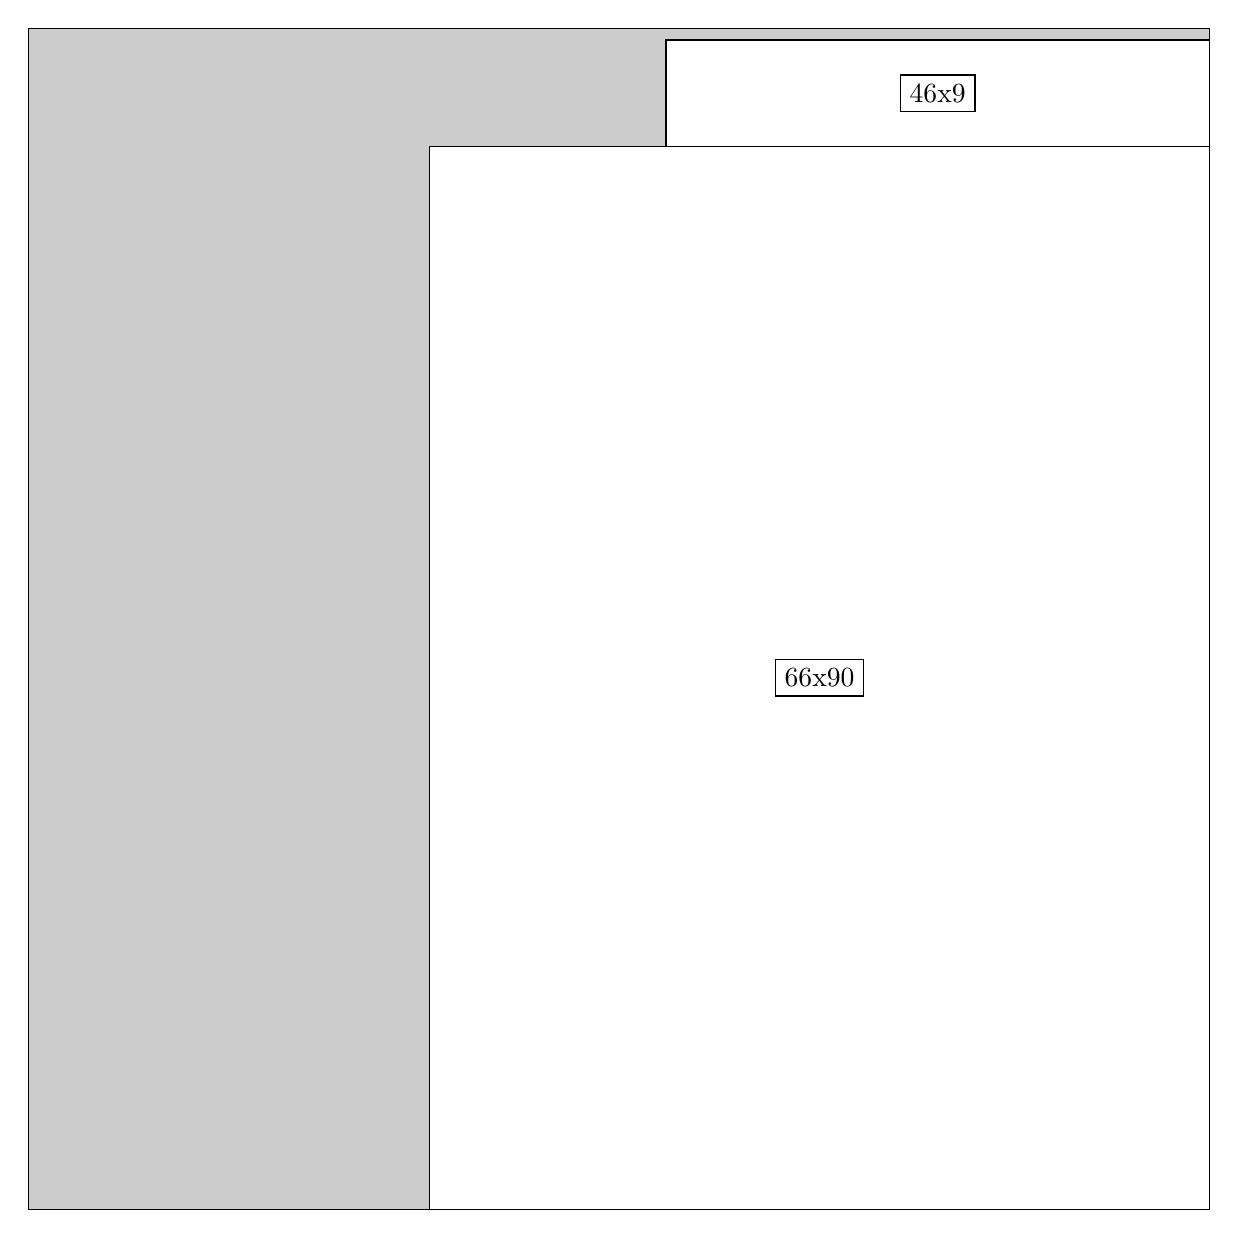
\begin{tikzpicture}[shorten >=1pt,scale=1.0,every node/.style={scale=1.0},->]
\tikzstyle{vertex}=[circle,fill=black!25,minimum size=14pt,inner sep=0pt]
\filldraw[fill=gray!40!white, draw=black] (0,0) rectangle (15.0,15.0);
\foreach \name/\x/\y/\w/\h in {66x90/5.1/0.0/9.9/13.5,46x9/8.1/13.5/6.8999999999999995/1.3499999999999999}
\filldraw[fill=white!40!white, draw=black] (\x,\y) rectangle node[draw] (\name) {\name} ++(\w,\h);
\end{tikzpicture}


w =66 , h =90 , x =34 , y =0 , v =5940
\par
w =46 , h =9 , x =54 , y =90 , v =414
\par
\newpage


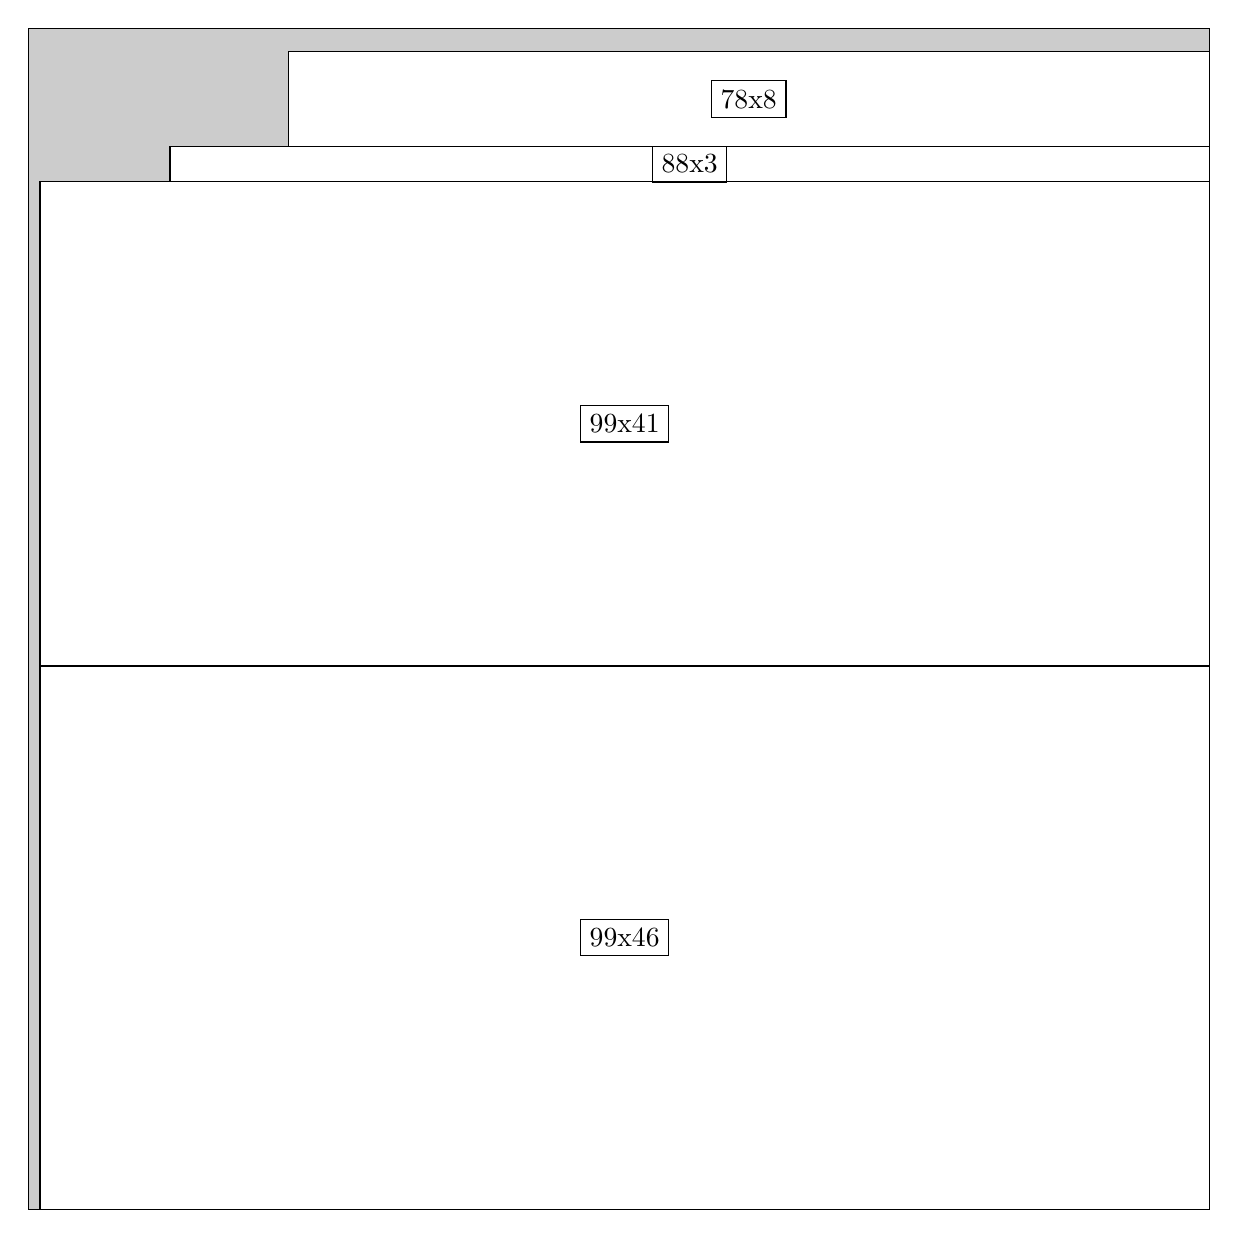
\begin{tikzpicture}[shorten >=1pt,scale=1.0,every node/.style={scale=1.0},->]
\tikzstyle{vertex}=[circle,fill=black!25,minimum size=14pt,inner sep=0pt]
\filldraw[fill=gray!40!white, draw=black] (0,0) rectangle (15.0,15.0);
\foreach \name/\x/\y/\w/\h in {99x46/0.15/0.0/14.85/6.8999999999999995,99x41/0.15/6.8999999999999995/14.85/6.1499999999999995,88x3/1.7999999999999998/13.049999999999999/13.2/0.44999999999999996,78x8/3.3/13.5/11.7/1.2}
\filldraw[fill=white!40!white, draw=black] (\x,\y) rectangle node[draw] (\name) {\name} ++(\w,\h);
\end{tikzpicture}


w =99 , h =46 , x =1 , y =0 , v =4554
\par
w =99 , h =41 , x =1 , y =46 , v =4059
\par
w =88 , h =3 , x =12 , y =87 , v =264
\par
w =78 , h =8 , x =22 , y =90 , v =624
\par
\newpage


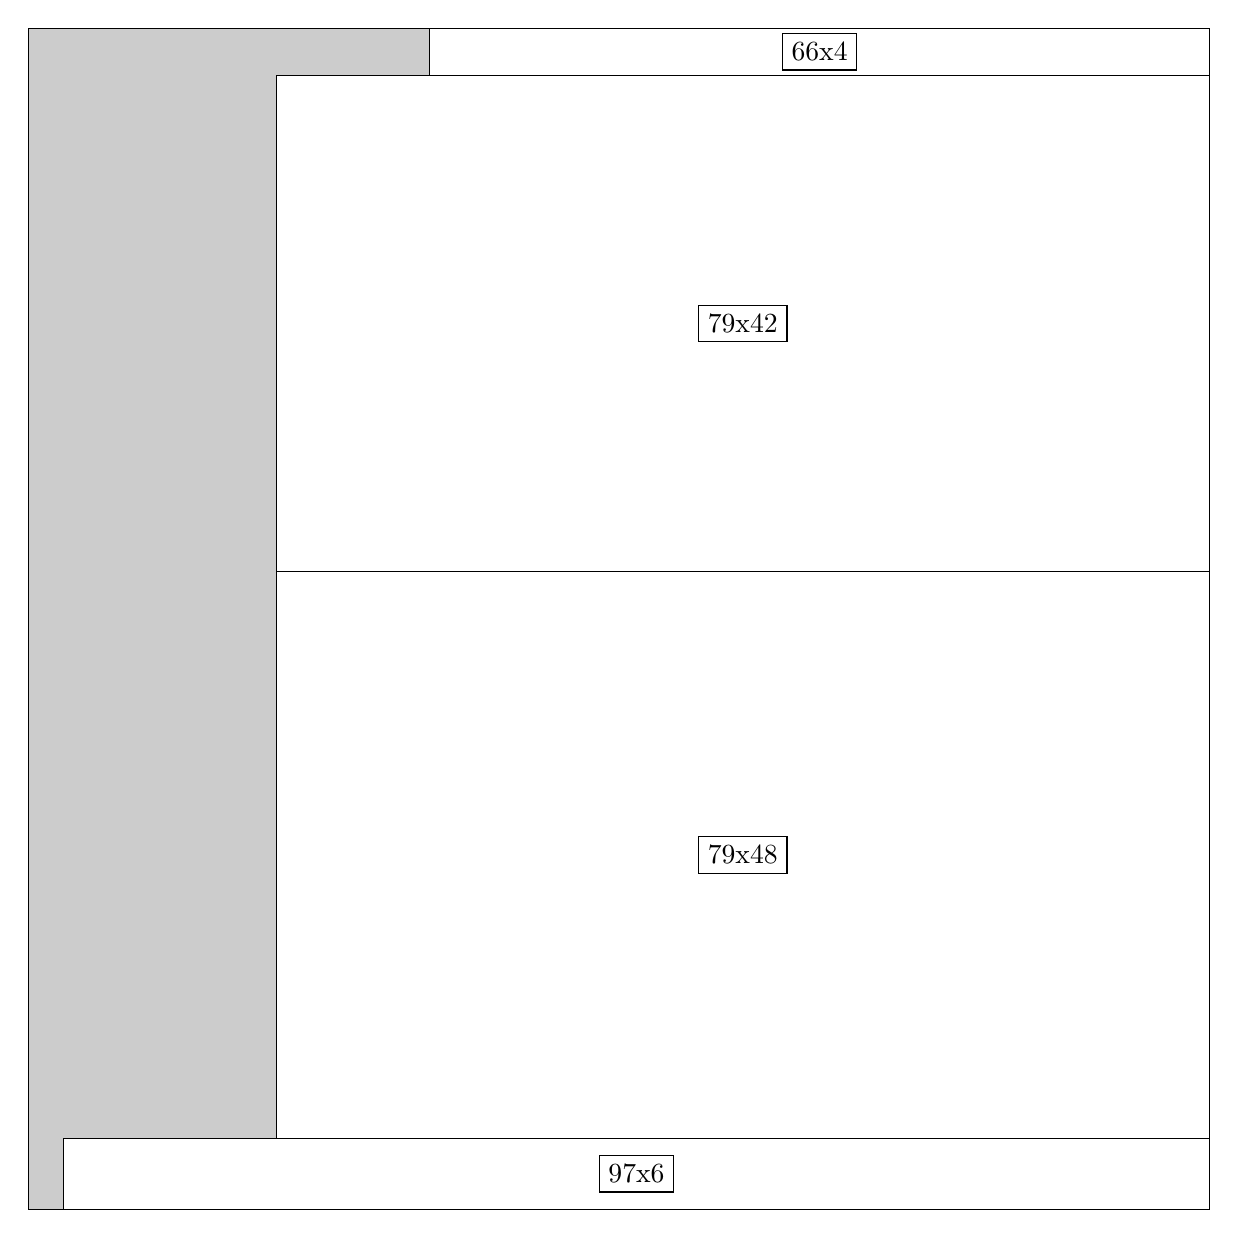
\begin{tikzpicture}[shorten >=1pt,scale=1.0,every node/.style={scale=1.0},->]
\tikzstyle{vertex}=[circle,fill=black!25,minimum size=14pt,inner sep=0pt]
\filldraw[fill=gray!40!white, draw=black] (0,0) rectangle (15.0,15.0);
\foreach \name/\x/\y/\w/\h in {97x6/0.44999999999999996/0.0/14.549999999999999/0.8999999999999999,79x48/3.15/0.8999999999999999/11.85/7.199999999999999,79x42/3.15/8.1/11.85/6.3,66x4/5.1/14.399999999999999/9.9/0.6}
\filldraw[fill=white!40!white, draw=black] (\x,\y) rectangle node[draw] (\name) {\name} ++(\w,\h);
\end{tikzpicture}


w =97 , h =6 , x =3 , y =0 , v =582
\par
w =79 , h =48 , x =21 , y =6 , v =3792
\par
w =79 , h =42 , x =21 , y =54 , v =3318
\par
w =66 , h =4 , x =34 , y =96 , v =264
\par
\newpage


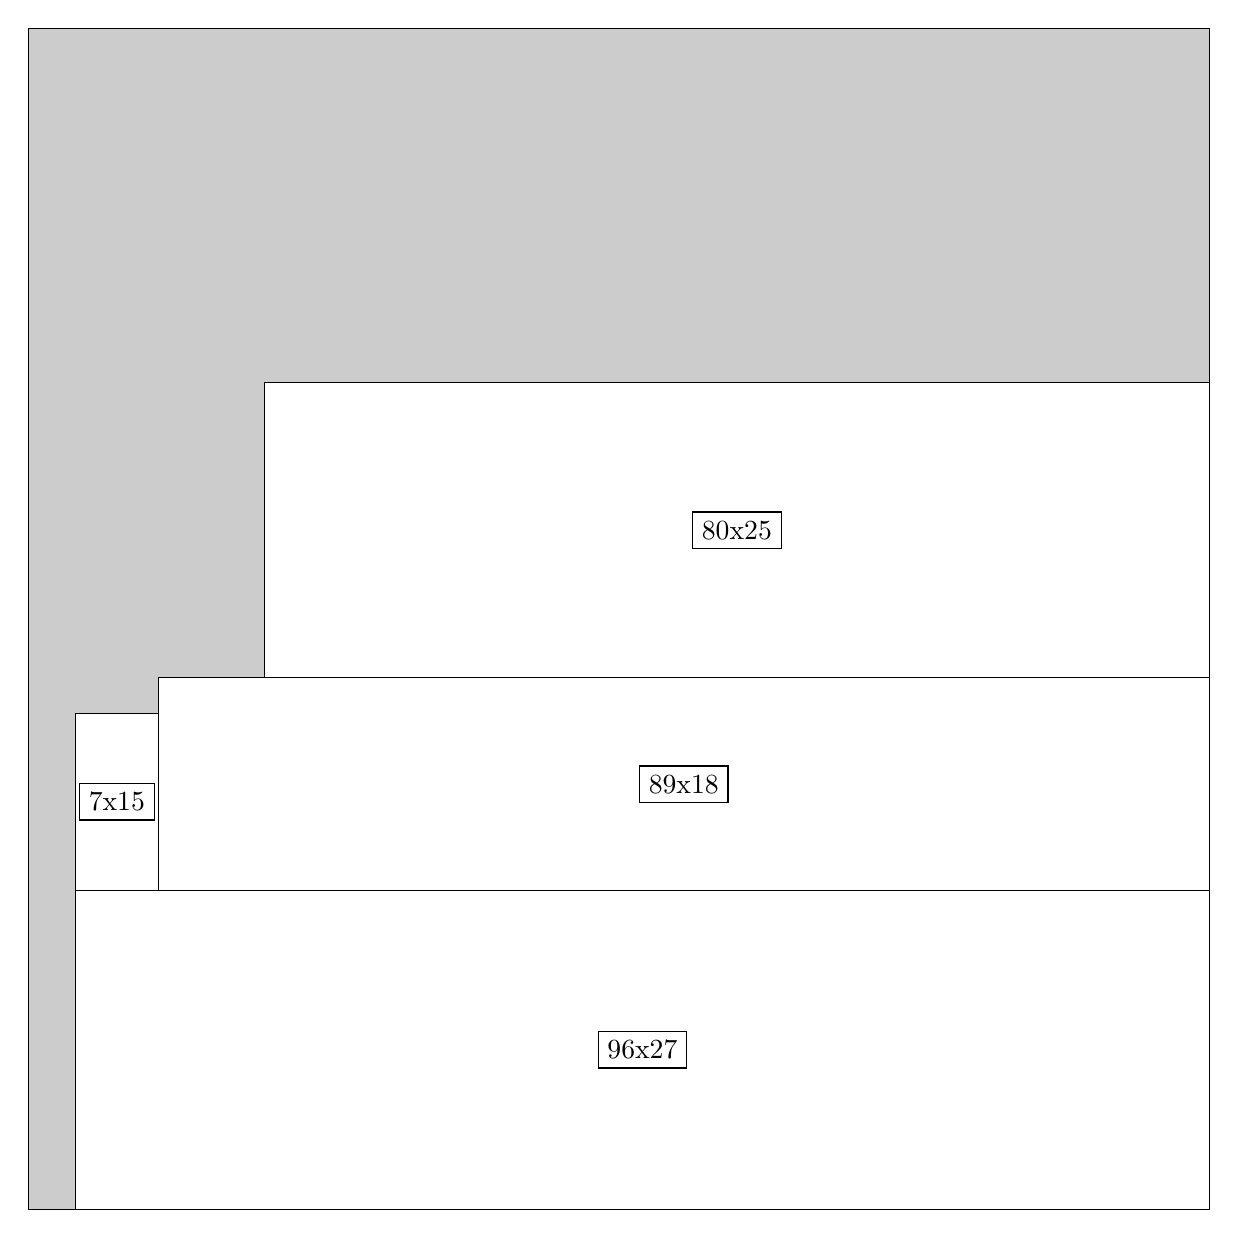
\begin{tikzpicture}[shorten >=1pt,scale=1.0,every node/.style={scale=1.0},->]
\tikzstyle{vertex}=[circle,fill=black!25,minimum size=14pt,inner sep=0pt]
\filldraw[fill=gray!40!white, draw=black] (0,0) rectangle (15.0,15.0);
\foreach \name/\x/\y/\w/\h in {96x27/0.6/0.0/14.399999999999999/4.05,89x18/1.65/4.05/13.35/2.6999999999999997,7x15/0.6/4.05/1.05/2.25,80x25/3.0/6.75/12.0/3.75}
\filldraw[fill=white!40!white, draw=black] (\x,\y) rectangle node[draw] (\name) {\name} ++(\w,\h);
\end{tikzpicture}


w =96 , h =27 , x =4 , y =0 , v =2592
\par
w =89 , h =18 , x =11 , y =27 , v =1602
\par
w =7 , h =15 , x =4 , y =27 , v =105
\par
w =80 , h =25 , x =20 , y =45 , v =2000
\par
\newpage


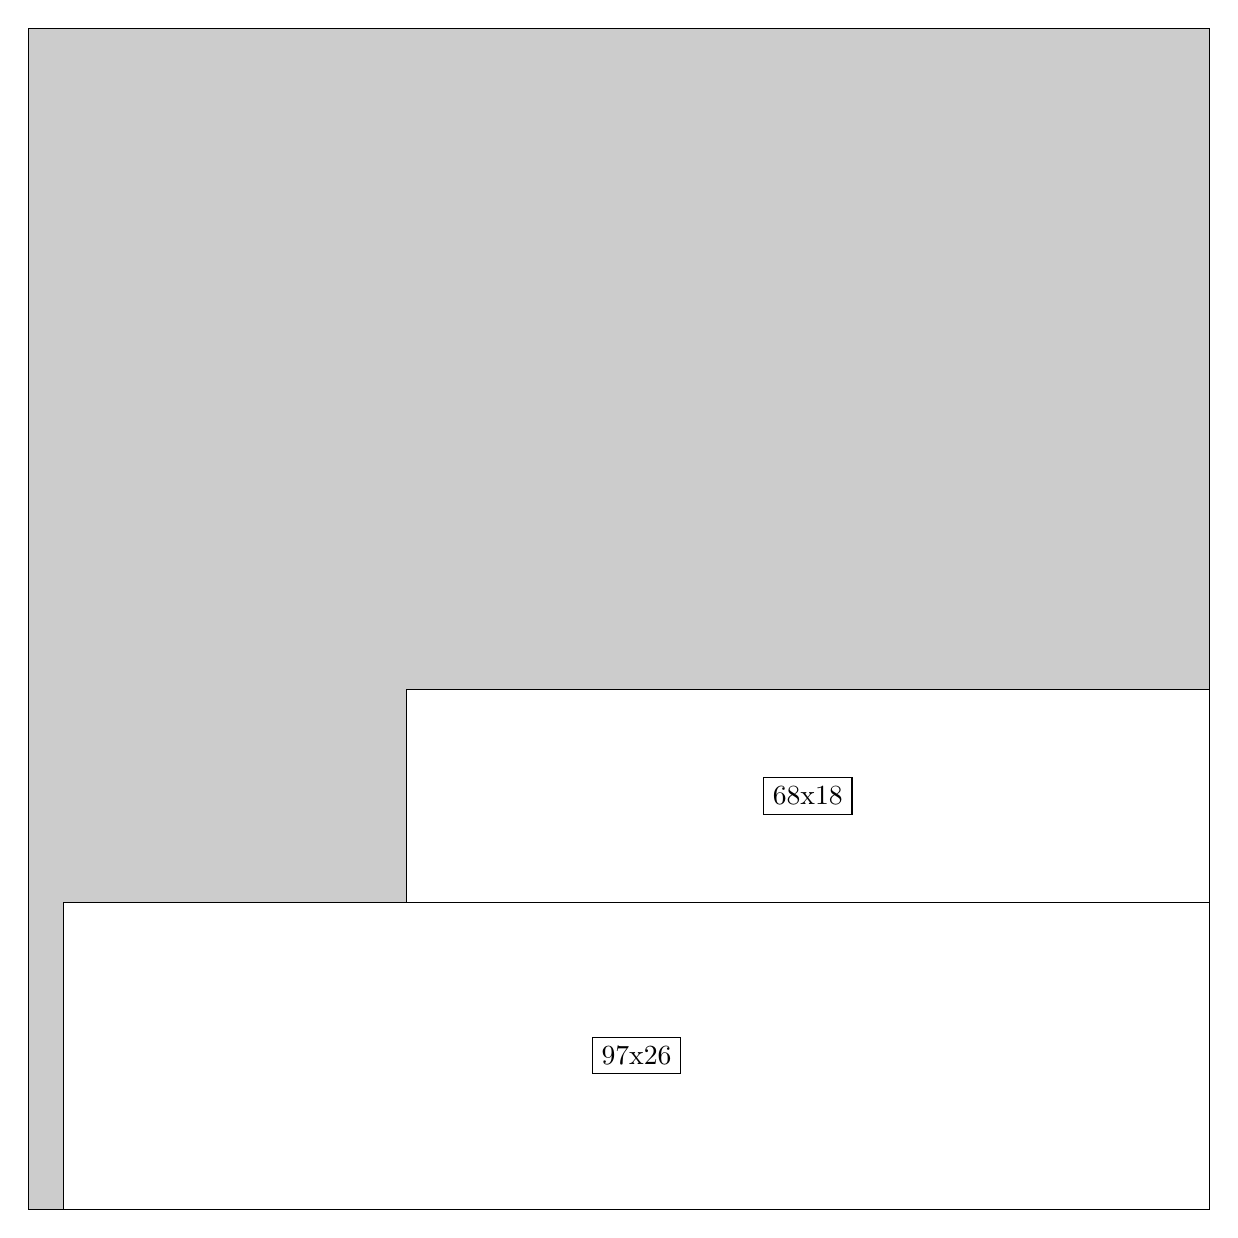
\begin{tikzpicture}[shorten >=1pt,scale=1.0,every node/.style={scale=1.0},->]
\tikzstyle{vertex}=[circle,fill=black!25,minimum size=14pt,inner sep=0pt]
\filldraw[fill=gray!40!white, draw=black] (0,0) rectangle (15.0,15.0);
\foreach \name/\x/\y/\w/\h in {97x26/0.44999999999999996/0.0/14.549999999999999/3.9,68x18/4.8/3.9/10.2/2.6999999999999997}
\filldraw[fill=white!40!white, draw=black] (\x,\y) rectangle node[draw] (\name) {\name} ++(\w,\h);
\end{tikzpicture}


w =97 , h =26 , x =3 , y =0 , v =2522
\par
w =68 , h =18 , x =32 , y =26 , v =1224
\par
\newpage


\end{document}